%include part: see main.beamer.tex and main.article.tex
%include common packages and settings
\usepackage{etex} %эта магическая херь избавляет от переполнения регистров TeX а!!!

\mode<article>{\usepackage{fullpage}}
\mode<presentation>{
    \usetheme{Madrid} %%Boadilla,Madrid,AnnArbor,CambridgeUS,Malmoe,Singapore,Berlin
    \useoutertheme{shadow}
} 

\usepackage[utf8]{inputenc}
\usepackage[russian]{babel}
\usepackage{indentfirst}
\usepackage{graphicx}

\usepackage{amsmath}
\usepackage{amsfonts}
\usepackage{amsthm}
\usepackage{algorithm}
\usepackage{algorithmic}

\usepackage[all]{xy}

\date{Лекция по дисциплине <<дискретная математика>>\\(\today)}
\author[М.~М.~Шихов]{Михаил Шихов \\ \texttt{\underline{m.m.shihov@gmail.com}}}

%для рисования графов пакетом xy-pic
\entrymodifiers={++[o][F-]}

%для псевдокода алгоритмов (algorithm,algorithmic)
\renewcommand{\algorithmicrequire}{\textbf{Вход:}}
\renewcommand{\algorithmicensure}{\textbf{Выход:}}
\renewcommand{\algorithmiccomment}[1]{// #1}
\floatname{algorithm}{Псевдокод}



\title[Регулярные множества]{Регулярные множества}


\begin{document}

%титул и содержание статьи
\mode<article>{\maketitle\tableofcontents}

%титул и содержание презентации
\frame<presentation>{\titlepage}
\begin{frame}<presentation>
    \frametitle{Содержание}
    \tableofcontents
\end{frame}


\section{Регулярные множества и выражения}

\subsection{Основные определения}

\begin{frame}
    \frametitle{Элементы регулярного множества}
    \framesubtitle{Цепочки символов (слов) в алфавите $T$}
    
    \begin{definition}
        \begin{itemize}
            \item $T$ --- \alert{алфавит} букв. $a\in T$, $a$ --- \alert{буква}, \alert{символ}.
            \item \alert{Цепочка}, \alert{слово} в алфавите $T$--- упорядоченная последовательность букв $T$.
            \item \alert{Префикс}, \alert{приставка} слова $\omega$ --- это цепочка $\omega_1$, если $\omega=\omega_1\omega_2$.
            \item \alert{Постфикс}, \alert{окончание} --- это $\omega_2$ в $\omega=\omega_1\omega_2$.
            \item \alert{Пустая} цепочка $\varepsilon$. Для любой $\omega$ справедливо $\omega=\varepsilon\omega=\omega\varepsilon$.
        \end{itemize}
    \end{definition}
    \begin{example}[Конкатенация цепочек. $\omega_1=abc$, $\omega_2=def$]
        \[
            \begin{array}{l}
                \omega_1\omega_2=abcdef,\\
                \omega_2\omega_1=defabc,\\
                \varepsilon\omega_1={\varepsilon}abc=abc.
            \end{array}
        \]
    \end{example}
\end{frame}


\begin{frame}
    \frametitle{Конкатенация регулярных множеств}
    
    \begin{definition}
        \alert{Конкатенацией} множеств цепочек $A$ и $B$, будет множество 
        \[
            AB=\{\omega_A \omega_B |\omega_A\in A\land \omega_B\in B\}.
        \]
    \end{definition}
    
    \begin{example}[$A=\{a,bb,ccc\}$, $B=\{1,22\}$]
        \[
            AB=\uncover<2>{\{a1,a22,bb1,bb22,ccc1,ccc22\}}
        \]
    \end{example}
\end{frame}

\begin{frame}
    \frametitle{Возведение регулярного множества в степень}
    
    \begin{definition}
        \alert{Возведением в степень} $n$ (где $n\geq 0$) множества $A$ будем называть:
        \[
            A^n=
            \begin{cases}
                AA^{(n-1)},         &\text{при } $n>1$,\\
                \{\varepsilon\},    &\text{при } $n=0$.
            \end{cases}
        \]            
        Другими словами 
        \(
            A^n=\underbrace{AA\cdots A}_{n-\text{раз}}.
        \)
    \end{definition}

    \begin{example}
        \[
            \begin{split}
                \{0,1\}^3=\uncover<2>{
                    \{00,01,10,11\}\{0,1\}=\\
                    =\{000,001,010,011,100,101,110,111\}.
                }
            \end{split}
        \]
    \end{example}
\end{frame}


\subsection{Регулярное множество}

\begin{frame}
    \frametitle{Определение регулярного множества}
    
    Регулярным множеством в алфавите $T$ является:
    \begin{enumerate}
        \item $\emptyset$
        \item $\{\varepsilon\}$
        \item $\{s\}$, где $s\in T$
        \item Если $A$ и $B$ --- регулярные множества в алфавите $T$.
        \begin{enumerate}
            \item $A\cup B$.
            \item $AB$.
            \item $A^*$, где
                \[A^*=\bigcup_{i=0}^{\infty}A^i.\]
        \end{enumerate}
    \end{enumerate}
    \begin{example}[$A=\{a,b\}$]
        \[A^*=\{\varepsilon,a,b,aa,ab,ba,bb,aaa,aab,aba,abb,baa,bab,bba,\ldots\}\]
    \end{example}
\end{frame}


\subsection{Регулярное выражение}

\begin{frame}
    \frametitle{Определение регулярного выражения}
    \framesubtitle{Регулярное выражение задает регулярное множество}
    
    Регулярному выражению соответствует ($\mapsto$) регулярное множество.
    \begin{enumerate}
        \item $\emptyset\mapsto\emptyset$.
        \item $\varepsilon\mapsto\{\varepsilon\}$.
        \item $s\mapsto\{s\}$, где $s\in T$.
        \item Если $a$ и $b$ --- регулярные выражения, $a\mapsto A$ и $b\mapsto B$.
        \begin{enumerate}
            \item $(a|b)\mapsto (A\cup B)$. Объединение.
            \item $(ab)\mapsto (AB)$. Конкатенация.
            \item $(a^*)\mapsto (A^*)$. Итерация.
        \end{enumerate}
    \end{enumerate}
    
    Приоритеты: <<итерация>> $>$ <<конкатенация>> $>$ <<объединение>>. 
    
    Например: $d|abc^*\Leftrightarrow(d|((ab)(c^*)))$
\end{frame}

\begin{frame}
    \frametitle{Примеры регулярных выражений}

    Регулярному выражению будут соответствовать цепочки
    \begin{itemize}
        \item $1|a(b|c|d)\mapsto\uncover<2->{\{1,ab,ac,ad\}}$
        \item $0(0|1|2|3|4|5|6|7)^*\mapsto\uncover<3->{\text{Натуральные числа в 8 СС}}$
        \item $(\textit{паша}|\textit{саша})+(\textit{маша}|\textit{даша})=\textit{Л}\ldots\mapsto\uncover<4->{\text{Любовный четырёхугольник}}$
        \item $(\textit{це}|\varepsilon)\textit{почк}(\textit{а}|\textit{и}|\textit{е}|\textit{у}|\textit{ой})\mapsto\uncover<5->{\text{Падежи почки с цепочкой}}$
    \end{itemize}
\end{frame}


\section{FYI: PCRE}

\begin{frame}
    \frametitle{PCRE}
    \framesubtitle{Perl Compatible Regular Expressions}
    
    В составе PCRE выделяют:
    \begin{itemize}
        \item одиночные символы; 
        \item классы символов; 
        \item альтернативы; 
        \item квантификаторы; 
        \item мнимые символы; 
        \item ссылки на найденный текст;
        \item и т.д.
    \end{itemize}
\end{frame}


\subsection{Поиск по шаблону}

\begin{frame}[fragile]
    \frametitle{PCRE}
    \framesubtitle{Одиночный символ}
    
    Любой одиночный символ $s$ в составе PCRE соответствует сам себе, если только он не является служебным символом (спецсимволом), играющим особую роль. 
    
    Служебными символами являются <<\verb"\">>, <<\verb"|">>, <<\verb"(">>, <<\verb")">>, <<\verb"[">>, <<\verb"]">>, <<\verb"{">>, <<\verb"}">>, <<\verb"*">>, <<\verb"+">>, <<\verb"^">>, <<\verb"$">>, <<\verb"?">> и <<\verb".">>. 
    
    Если необходимо, чтобы служебный символ соответствовал самому себе, то перед ним нужно поставить символ <<\verb"\">>. Регулярное выражение, производящее поиск символа <<\verb"\">> в тексте будет выглядеть так <<\verb"\\">>.
\end{frame}

\begin{frame}[fragile]
    \frametitle{PCRE}
    \framesubtitle{Предопределенные классы и символы, ввод которых затруднён}
    
    \begin{itemize}
        \item{} <<\verb"\d">> – любая десятичная цифра;
        \item{} <<\verb"\D">> – любой символ, кроме десятичной цифры;
        \item{} <<\verb"\s">> – любой из символов-разделителей;
        \item{} <<\verb"\S">> – любой символ, за исключением пробельного;
        \item{} <<\verb"\w">> – алфавитно-цифровой символ и знак <<\verb"_">>;
        \item{} <<\verb"\W">> – любой символ, но не <<\verb"\w">>;
        \item{} <<\verb"\r">>  – символ перевода каретки \verb"<CR>";
        \item{} <<\verb"\n">>  – символ новой строки \verb"<LF>";
        \item{} <<\verb"\R">>  – независимый от платформы разделитель строк;
        \item{} <<\verb"\xHH">> – символ ASCII с кодом из двух шестнадцатеричных (\verb"HH") цифр;
        \item{} <<\verb"\uHHHH">> – символ Unicode с кодом из четырех шестнадцатеричных (\verb"HHHH") цифр.
    \end{itemize}
\end{frame}
%ввод Alt+<код на цифровой клавиатуре(10 сс)> попробовать поиск \x98 для кода буквы "b".

\begin{frame}[fragile]
    \frametitle{PCRE}
    \framesubtitle{Точка}

    Спецсимвол точка <<\verb".">> соответствует любому символу, за исключением разделителя строк.
\end{frame}

\begin{frame}[fragile]
    \frametitle{PCRE}
    \framesubtitle{Классы символов}
    
    \alert{Класс} определяет соответствие одному символу из множества. Класс --- это список символов, заключенный в квадратные скобки <<\verb"[">>, <<\verb"]">>. Можно указать как отельные символы, так и диапазон. Диапазон задается двумя крайними символами диапазона, разделенными тире. Если требуется указать тире, то перед ним ставится символ <<\verb"\">>. 
    
    Например.
    \begin{itemize}
        \item{} <<\verb"[abcde]">> --- любая из букв <<\verb"а">>, <<\verb"b">>, <<\verb"c">>, <<\verb"d">>, <<\verb"e">>. Более кратко: <<\verb"[a-e]">>.
        \item Равнозначны: <<\verb"[\-0123456789]">>, <<\verb"[\-0-9]">> и <<\verb"[\-\d]">>.
    \end{itemize}
     Если сразу после открывающей квадратной скобки следует спецсимвол <<\verb"^">>, то будет выполняться поиск соответствия символу, не входящему в класс. Например, <<\verb"[^a-e]">> --- любой символ, \emph{кроме}: <<\verb"а">>, <<\verb"b">>, <<\verb"c">>, <<\verb"d">>, <<\verb"e">>.
\end{frame}


\begin{frame}[fragile]
    \frametitle{PCRE}
    \framesubtitle{Альтернативы}
    
    \alert{Альтернативa} соответствуют операции объединения в формальном определении регулярных выражений. Альтернативные регулярные выражения разделяются спецсимволом <<\verb"|">> и обычно заключаются в круглые скобки.

    Альтернатива <<\verb"(a|b)">> соответствует либо шаблону <<\verb"a">>, либо <<\verb"b">>.
    
    Например.
    \begin{enumerate}
        \item Двоичная цифра: <<\verb"(0|1)">>.
        \item Троичная цифра: <<\verb"(0|1|2)">>.
        \item Любая тетрада:  <<\verb"(0|1)(0|1)(0|1)(0|1)">>.
    \end{enumerate}
\end{frame}


\begin{frame}[fragile]
    \frametitle{PCRE}
    \framesubtitle{Квантификаторы}
    
    \alert{Квантификаторы} ставятся после регулярного выражения и определяют количество повторений шаблона. Выделяют следующие квантификаторы:
    \begin{itemize}
        \item{} <<\verb"*">> --- ноль или несколько повторов;
        \item{} <<\verb"+">> --- один или несколько повторов;
        \item{} <<\verb"?">> --- ноль или один повтор;
        \item{} <<\verb"{n}">> --- ровно \verb"n" повторов (\verb"n" --- десятичное число);
        \item{} <<\verb"{n,}">> --- по крайней мере \verb"n" повторов;
        \item{} <<\verb"{n,m}">> --- от \verb"n" до \verb"m" повторов.
    \end{itemize}
\end{frame}

\begin{frame}[fragile]
    \frametitle{PCRE}
    \framesubtitle{Жадность и лень}
    
    По умолчанию квантификаторы <<\verb"*">>, <<\verb"+">>, <<\verb"?">>, <<\verb"{n,}">>, <<\verb"{n,m}">> являются \alert{жадными} (greedy): они выделят по возможности самый длинный фрагмент из всех возможных. 
    
    Например, при поиске в тексте <<\verb"aaaaaaaaaa">> шаблону <<\verb"a*a">> будет соответствовать весь текст. Сделать квантификаторы \alert{ленивыми} (lazy) можно, поставив после них знак вопроса <<\verb"?">>. Тогда в приведенном примере для ленивого варианта <<\verb"a*?a">> результатом поиска будет одна буква <<\verb"a">>.    
\end{frame}


\begin{frame}[fragile]
    \frametitle{PCRE}
    \framesubtitle{Мнимые символы}
    
    \alert{Мнимые символы} не соответствуют символам текста! Они соответствуют выполнению определенного условия (assertion), например:
    \begin{itemize}
        \item{} <<\verb"^">> --- начало строки текста;
        \item{} <<\verb"$">> --- конец строки или позиция перед символом начала новой строки;
        \item{} <<\verb"\b">> --- граница слова;
        \item{} <<\verb"\B">> --- отсутствие границы слова.
    \end{itemize}
\end{frame}


\subsection{Ссылки и <<умные>> замены}

\begin{frame}[fragile]
    \frametitle{PCRE}
    \framesubtitle{Сылки на фрагменты шаблона}
    
    Каждому выражению, заключенному в скобки соответствует переменная с определенным номером. Так как части регулярного выражения заключенные в скобки могут быть вложенными, то нумеруются они с единицы по открывающим скобкам, слева направо. В 0-й переменной содержится текст соответствующий шаблону целиком.
    
    Например, если задано регулярное выражение 
    \begin{center}
        <<\verb"(\w(\w(\w)))((\w)(\w))">>
    \end{center}
    и текст <<\verb"ABCDE">>, то значения переменных будут: \verb"$0"=<<\verb"ABCDE">>, \verb"$1"=<<\verb"ABC">>, \verb"$2"=<<\verb"BC">>, \verb"$3"=<<\verb"C">>, \verb"$4"=<<\verb"DE">>, \verb"$5"=<<\verb"D">>, \verb"$6"=<<\verb"E">>. 
\end{frame}

\begin{frame}[fragile]
    \frametitle{PCRE}
    \framesubtitle{Поиск со ссылками на найденные фрагменты}
    
    Иногда в процессе поиска нужно сослаться на подстроку текста, для которой уже получено совпадение с некоторой частью регулярного выражения. 
    
    Для этого необходимую часть следует заключить в круглые скобки и сослаться на нее. Для этого перед номером переменной достаточно поставить <<\verb"\">>. 
    
    Например, если необходимо найти целое положительное число, являющееся значением элемента XML\footnote{Например: \verb"some text <age>100</age> some text"}, то можно задать такое выражение: <<\verb"<(\w+)>\d+</\1>">>. В переменной \verb"\1" будет содержаться текст, соответствующий регулярному выражению <<\verb"(\w+)">>.    
\end{frame}

\begin{frame}[fragile]
    \frametitle{PCRE}
    \framesubtitle{Замены}
    
    С помощью ссылок на фрагменты текста, соответствующего шаблону регулярного выражения очень удобно выполнять самые нетривиальные замены в тексте. Например, переставить байты в 32 битном шестнадцатеричном числе в обратном порядке можно так: заменить текст, соответствующий регулярному выражению 
    \begin{center}
        <<\verb"0x([0-9A-F]{2})([0-9A-F]{2})([0-9A-F]{2})([0-9A-F]{2})">>
    \end{center}
    на текст\footnote{Здесь мы обращаемся к переменной с номером \verb"n" так: <<\verb"\$1">>} <<\verb"0x$4$3$2$1">>. Число <<\verb"0x01ABCDEF">> будет заменено на <<\verb"0xEFCDAB01">>.
\end{frame}
    
\begin{frame}
    \frametitle{PCRE}
    \framesubtitle{Есть в любом хорошем текстовом редакторе}

    IDE Eclipse:
    \begin{center}
        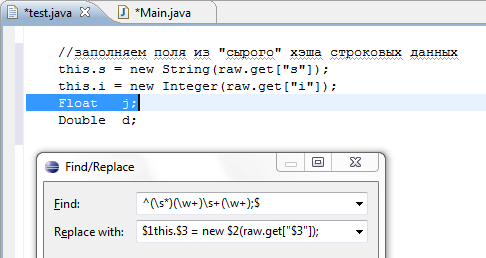
\includegraphics[width=.9\textwidth]{fig/eclipseIde}
    \end{center} 
\end{frame}


\appendix

\begin{frame}[fragile]
    \frametitle{PCRE-навыки}
    \framesubtitle{Редактор с открытым кодом jEdit}

    
    \begin{enumerate}
        \item{} <<\verb"Alt+48">>=<<\verb"0">>. Найти символ \verb"3" по коду.
        \item Найти имя переменной в тексте.
        \item Классы \verb"[a-d]+" и \verb"[^a-d]+", на тексте \verb"abc123abc123". Проверить на жадность. Проверить квантификаторы вида \verb"{n,m}".
        \item Альтернатива \verb"(це|)почк(а|и|е|у|ой)", на почках и цепочках.
        \item \verb"имя:тип" $\Rightarrow$ \verb"x.имя=new тип(hash['имя'])".
\begin{verbatim}        
    firstname:String
    lastname:String
    middlename:String
    birthday:Date
    adress:String
    place:Coordinate
\end{verbatim}        
        \item Найти определение функции одного аргумента в паскале.
    \end{enumerate} 
\end{frame}

\begin{frame}[fragile,allowframebreaks]
    \frametitle{PCRE-практикум}

    \begin{enumerate}
        \item Организуйте в тексте поиск чисел. Примеры чисел: \verb"0", \verb"-5", \verb"0.1", \verb"-2.24", \verb"-2.123e-15", \verb"-31.123E+7". Запись числа \verb"-31.123E-7" называется \emph{научной} нотацией и её следует понимать так: $-31.123\cdot 10^{-7}$.
        
        \item Найдите в тексте e-mail адреса. Адреса рунета. Замените адрес предложением <<в адресе <адрес> имя пользователя:<имя>, хост:<хост>, домен:<домен>>>
        
        \item Даты у разных народов пишутся по-разному. Например, в России принято писать сначала день, потом месяц, потом год: <<\verb"29.02.1982">>, <<\verb"29/02/1982">>. В США, например, даты пишут в таком порядке: месяц, день, год. Выполните замены американских дат российскими, учтя, что разделителями могут быть точка, дефис и косая черта. Числа, соответствующие дням и месяцам не обязательно дополняются ведущим нулем: <<\verb"1.1.2011">>. В тексте не встретится сокращенных записей для года (иногда пишут \verb"82" вместо \verb"1982").
        
        \item В базе данных скопилось множество номеров телефонов одного города. Пусть это будет Киров с международным кодом \verb"8(8332)". В свое время под номер была отведена строка, и операторы вводили номера телефонов, сообразуясь со своими эстетическими пристрастиями: \verb"8-8332-123456", \verb"8 8332 12 34 56", \verb"8-8332-123-456", \verb"8-8332-12-34-56", \verb"8(8332)12 34 56". И даже без кода: \verb"12 34 56", \verb"123-456". Пора положить конец хаосу. Да будет единый: \verb"8(8332)XX-XX-XX".
    \end{enumerate} 
\end{frame}

\begin{frame}
    \frametitle{В заключение}
    
    В своё время регулярные выражения были прорывом в технике обработки текстов. И они не теряют своих позиций со временем. Регулярные выражения являются частью синтаксиса многих языков программирования\footnote{Например, perl}, в остальных же языках регулярные выражения доступны через функции стандартных библиотек. Практически все достойные внимания среды разработки поддерживают поиск и замену на основе регулярных выражений. Почерпнуть информацию о регулярных множествах и выражениях можно из \cite{bib:serebryakov:programminglang}.
\end{frame}

\begin{frame}[allowframebreaks]{Библиография}
    \bibliographystyle{gost780u}
    \bibliography{./../../bibliobase}
\end{frame}

\end{document}